\documentclass[12pt,a4paper]{report}
\usepackage[top=2.5cm, bottom=2.5cm, left=2.5cm, right=2.5cm]{geometry}

% Diff�rentes options pour la classe :
% - taille de la fonte    : 10pt, 11pt, 12pt
% - recto ou recto-verso    : oneside, twoside
% - stade de d�veloppement    : draft, final


\usepackage[English]{babel}
\usepackage[latin1]{inputenc}    % Pour utiliser les lettres accentu�es

%\usepackage[utf8]{inputenc}%           gestion des accents (source)
\usepackage[T1]{fontenc}%              gestion des accents (PDF)
%\usepackage[francais,english]{babel}%          gestion du fran�ais
\usepackage{textcomp}%                 caract�res additionnels

\usepackage[pdftex]{graphicx}
\usepackage{setspace}
\usepackage{hyperref}
\usepackage[french]{varioref}
\usepackage{fancyhdr}
\usepackage{color}
\usepackage{colortbl}
\usepackage{amsmath}
\usepackage{ifpdf} % part of the hyperref bundle
\usepackage{array}


%\usepackage{abstract}


 % set fonts for nicer pdf view
 \IfFileExists{lmodern.sty}{\usepackage{lmodern}}{}


\pagestyle{fancy}
\fancyhead[L]{}
\fancyhead[C]{}
\fancyhead[R]{\nouppercase\rightmark}


\fancyfoot[L]{}
\fancyfoot[C]{}
\fancyfoot[R]{\textbf{\thepage}}

% D�but du document
\begin{document}

%%%%%%%%%%%%%%%%%%%%%%%%%%%%%%%%%%%%%%%%%
% University Assignment Title Page 
% LaTeX Template
% Version 1.0 (27/12/12)
%
% This template has been downloaded from:
% http://www.LaTeXTemplates.com
%
% Original author:
% WikiBooks (http://en.wikibooks.org/wiki/LaTeX/Title_Creation)
%
% License:
% CC BY-NC-SA 3.0 (http://creativecommons.org/licenses/by-nc-sa/3.0/)
% 
% Instructions for using this template:
% This title page is capable of being compiled as is. This is not useful for 
% including it in another document. To do this, you have two options: 
%
% 1) Copy/paste everything between \begin{document} and \end{document} 
% starting at \begin{titlepage} and paste this into another LaTeX file where you 
% want your title page.
% OR
% 2) Remove everything outside the \begin{titlepage} and \end{titlepage} and 
% move this file to the same directory as the LaTeX file you wish to add it to. 
% Then add \input{./title_page_1.tex} to your LaTeX file where you want your
% title page.
%
%%%%%%%%%%%%%%%%%%%%%%%%%%%%%%%%%%%%%%%%%



\begin{titlepage}

\newcommand{\HRule}{\rule{\linewidth}{0.5mm}} % Defines a new command for the horizontal lines, change thickness here

\center % Center everything on the page
 
%----------------------------------------------------------------------------------------
%	HEADING SECTIONS
%----------------------------------------------------------------------------------------


\begin{minipage}[l]{0.2\columnwidth}

\includegraphics[width=3cm,height=2cm]{logo_istic.jpg}\\
\end{minipage}
\hfill
\begin{minipage}[l]{0.5\columnwidth}
\centering
\footnotesize
\textbf{\textsc{Tunisian Republic}}\\
\textbf{\textsc{Ministry of Higher Education\\
and Scientific Research}}\\
\medskip 
\textbf{\textsc{University of Carthage}}\\
\medskip 
\textbf{\textsc{Higher Institute of Information and Communication Technologies}}
\end{minipage}
\hfill
\begin{minipage}[l]{0.2\columnwidth}

\includegraphics[width=3cm,height=2cm]{universite-carthage.png}\\
\end{minipage}

\vskip2cm
\textsc{ \huge Internship Report}\\[0.5cm] % Minor heading such as course title\\


\textsc{\large Bachelors in Computer Engineering}\\[0.5 cm] % Minor heading such as course title\\

\textbf{Speciality : IOT And Embedded System}\\[0.3cm]

\vskip1cm%
\textit{Presented By}\\
\vskip0.5cm%
\textsc{\large Yahya Abulhaj}\\[0.5cm] % Minor heading
\smallskip

%----------------------------------------------------------------------------------------
%	TITLE SECTION
%----------------------------------------------------------------------------------------

\HRule \\[0.4cm]
\textcolor{red}{ \LARGE \bfseries Cloud Migration Research}\\[0.4cm] % Title of your document
\HRule \\[1cm]
%\vspace{0.5cm}
%\begin{center}
%\vspace{0.5cm}
%\begin{center}
{Made Within Linedata}\\
%\smallskip

\includegraphics[width=0.2\columnwidth]{Rapport ISTIC/linedata.jpg}\\
%\end{center}

\vskip1cm

%----------------------------------------------------------------------------------------
%	Supervisor SECTION
%----------------------------------------------------------------------------------------
 \begin{flushleft}
 \begin{center}
\textbf{Internship Period}: 13/06/2022 - 8/07/2022
\end{center}
%\smallskip
\vskip1cm
\begin{center}
Professional-Mentor: \textbf{Amal Dridi}, Specialist - Software Quality Assurance at Linedata\\
\end{center}
%\hfill
\begin{minipage}[c]{0.6\columnwidth}


\end{minipage}
%\begin{minipage}[c]{0.4\columnwidth}
%{\small Maitre-Assistant en Informatique}\\
%{\small Maitre-Assistant en Informatique}\\
%{\small Ing\'enieur}\\
%{\small Assistant en Informatique}
%\end{minipage}
 \end{flushleft}
 


%----------------------------------------------------------------------------------------
%	DATE SECTION
%----------------------------------------------------------------------------------------
\vskip2cm

{\large University year: 2022-2023}\\[3cm] 



\vfill % Fill the rest of the page with whitespace

\end{titlepage}
%\end{document}
\include{garde_sign_fin}
\newpage
\pagenumbering{roman}


\chapter*{Acknowledgment}
\addcontentsline{toc}{chapter}{Acknowledgment}
\newline

\textbf{Foremost}, I would like to express my sincere gratitude to my mentor Prof. Amal Dridi for the continuous support of my internship, for her patience, motivation, enthusiasm, and immense knowledge. \newline Her guidance helped me in all the time of expermimenting with the latest technologies and contributing to the company.
I could not have imagined having a better advisor and mentor for my summer internship.
\newline
It was a great privilege and honor to work and study under her guidance. I am extremely
grateful for what she has offered me. I would also like to thank her for the
friendship, empathy, and great sense of humor. 
\newline
I am overhelmed in all humbleness and gratefulness to acknowledge my depth to all those who have helped me to put these ideas, well above the level of simplicity and into something concrete.
\newline

Besides my advisor, I would like to thank the rest of the team at the Quality Assurance office: my manager, Marwan Sallem, Mohja Ben Amara for their encouragement, insightful comments, and hard questions.\newline
My sincere thanks also goes to Sandeep repswal, Sanjay Kulkarni from the india office for offering and enrolling me in their work and leading me to contribute on diverse exciting projects.
\newline

I would like to thank my mother who helped me a lot in gathering different information, collecting data and guiding me from time to time in making this state of mind and who i am. I am extremely grateful to her for her love, prayers, caring and
sacrifices for educating and preparing me for my future.
\newline

Also I express my thanks to my sister,
brother for their support and valuable prayers. My
Special thanks goes to my friend Kandarp, my online teammate for the
keen interest shown in career growth and collaboration to achieve success in life.
\newline
\textbf{Thank you, all.}
\vskip1.5cm
\begin{flushright}\LARGE
\bf{Yahya Abulhaj}
\end{flushright}

\chapter*{Abstract}
\addcontentsline{toc}{chapter}{Abstract}
\newline


\textbf{Cloud computing} is a pay-per-use model that enables available, convenient, on-demand network access to a shared pool of configurable computing resources (e.g., networks, servers, storage, applications, services) that can be rapidly provisioned and released with minimal management effort or interaction from service providers. This cloud model promotes availability and includes five key features, three delivery models, and four deployment models. Other leading cloud models, such as Microsoft Azure, Amazon Web Services, Google Cloud Platform & Salesforce.
I gathered some of the best quotes from the world of cloud computing and highly recommend you read them @ \href{https://devops.yahya-abulhaj.dev/}{DevOps.yahya-abulhaj.dev/}. 
\newline \newline
\newline \textbf{Entreprise Information:}\newline 
\textbf{Linedata} is a global publisher of value-added software, services, and data for the financial industry. Linedata has been assisting its clients, asset managers, institutional and alternative fund managers, fund administrators, and credit and financing institutions, in meeting their challenges for over 20 years through innovative and efficient solutions.
In today's world, quality is the buzzword, and without it, no organization can survive. Along with quality, we at Linedata. "Think Beyond" to go one step further and focus on solution delivery. We design processes that prioritize not only quality but also delivery, increasing the value to our global clients. I did not only get trained  on the latest technologies, but we the team we empower them to provide exciting solutions to our clients.
\newline \newline
\newline \textbf{Program And Opportunities:}\newline 
Linedata's success, in my opinion, is dependent on innovation and creativity. Currently navigating great fields of technology and will continue to do so.\newline 
\textbf{Software}, We create modular software platforms that are cloud-based and highly scalable due to the continuous delivery of new functionalities and modules, and I played a significant role in this.\newline 
\textbf{Analytics and data}, our AI and ML-powered data management services enable our customers to structure and exploit the right data from multiple sources without redundancy or additional cost.\newline 
\textbf{Services}, in key operational functions, our highly skilled experts supplement our clients' teams, delivering results, resilience, scalability, and efficiency.



\tableofcontents    % Table des mati�res       % Liste des tableaux
\pagenumbering{arabic}
\chapter*{ WEEKLY OVERVIEW}
\addcontentsline{toc}{chapter}{Timesheet}
\newline


\label{tab3}
\setlength{\arrayrulewidth}{0.5mm}
\setlength{\tabcolsep}{15pt}
\renewcommand{\arraystretch}{2.5}



\begin{tabular}{ |p{3cm}|p{3cm}|p{7cm}|  }
\hline

\hline
\end{tabular}



\begin{tabular}{ |p{3cm}|p{3cm}|p{7cm}|  }
\hline
\rowcolor[gray]{0.9}\multicolumn{3}{|c|}{ WEEK 1} \\
\hline
\textbf{DATE}& \textbf{DAYS}& \textbf{Activity}\\
\hline
13/06/2022 & Monday &Introduction to asset management. \\
\hline
14/06/2022  & Tuesday   & Setup VMS and deploy NGINX \\
\hline
15/06/2022  &Wednesday &  Setup SQL server \\
\hline
16/06/2022   &Thursday & Store, organize, and process data as required \\
\hline
17/06/2022   & Friday & Configure a Load balancing Solution \\
\hline
\end{tabular}


\begin{tabular}{ |p{3cm}|p{3cm}|p{7cm}|  }
\hline

\rowcolor[gray]{0.9}\multicolumn{3}{|c|}{ WEEK 2: Training} \\
\hline
\textbf{DATE}& \textbf{DAYS}& \textbf{Activity}\\
\hline
20/06/2022 & Monday &Fundamental Cloud Concepts for AWS \\
\hline
21/06/2022  & Tuesday   & Understanding AWS Core Services \\
\hline
22/06/2022  &Wednesday & Security and architecture on AWS \\
\hline
23/06/2022   &Thursday & Implement EC2, S3 and firewall \\
\hline
24/06/2022  & Friday & EXAM PREP: AZ-700 and AWS CCP \\
\hline
\end{tabular}
\begin{tabular}{ |p{3cm}|p{3cm}|p{7cm}|  }
\hline
\hline
\end{tabular} \\
\begin{tabular}{ |p{3cm}|p{3cm}|p{7cm}|  }
\hline
\rowcolor[gray]{0.9}\multicolumn{3}{|c|}{ WEEK 3} \\
\hline
\textbf{DATE}& \textbf{DAYS}& \textbf{Activity}\\
\hline
27/06/2022 & Monday &Configured Domain name server settings \\
\hline
28/06/2022  & Tuesday   & Create and configure Vnet gateway \\
\hline
29/06/2022  &Wednesday & Passed Microsoft Certified: Azure Network Engineer Associate \\
\hline
30/06/2022   &Thursday & Provision Infrastructure with Terraform: EC2, AWS Lambda \\
\hline
01/07/2022  & Friday & Maintained a Kubernetes cluster kubectl \\
\hline
\end{tabular}
\newline
\newline\begin{tabular}{ |p{3cm}|p{3cm}|p{7cm}|  }
\hline

\rowcolor[gray]{0.9}\multicolumn{3}{|c|}{ WEEK 4} \\
\hline
\textbf{DATE}& \textbf{DAYS}& \textbf{Activity}\\
\hline
04/07/2022 & Monday & Writing specifications and documentation for the server-side features \\
\hline
05/07/2022  & Tuesday   & Continuous deployment and continuous integration (CI/CD) management using Harness \\
\hline
06/07/2022  &Wednesday & Performance assessment and monitoring using
Nagios \\
\hline
07/07/2022   &Thursday & Cloud deployment and management of the project \\
\hline
08/07/2022  & Friday & Assistance with DevOps culture adoption, closure. \\
\hline
\end{tabular}
\newline


\chapter*{General Introduction}
\addcontentsline{toc}{chapter}{General Introduction}

The impact of cloud computing on industry and end users cannot be overstated: the ubiquitous presence of software that runs on cloud networks has transformed many aspects of daily life. Startups and businesses can reduce costs and expand their offerings by leveraging cloud computing rather than purchasing and managing their own hardware and software. Independent developers now have the ability to launch globally accessible apps and online services. Researchers can now share and analyze data on previously unimaginable scales. \textbf{Furthermore}, internet users can quickly access software and storage in order to create, share, and store digital media in quantities that far exceed the computing capacity of their personal devices.
\newline
Despite the growing popularity of cloud computing, many people are unaware of its specifics. What is the cloud, how does it work, and what are the advantages for businesses, developers, researchers, governments, healthcare practitioners, and students?.\newline
I had the opportunity to learn more about all of this as part of my internship. and I'll try to go into more detail in this report as best as i can.


\section{Define The Cloud }

Cloud computing is defined as follows by the National Institute of Standards and Technology (NIST), a non-regulatory agency of the United States Department of Commerce with the mission of advancing innovation:
\newline
a model for providing ubiquitous, convenient, on-demand network access to a shared pool of configurable computing resources (e.g., networks, servers, storage, applications, and services) that can be rapidly provisioned and released with minimal management effort or interaction from service providers

\subsection{Brief History}
Many aspects of cloud computing can be traced back to the 1950s, when universities and businesses rented out mainframe computer computation time. At the time, renting was one of the only ways to gain access to computing resources because computing technology was too large and expensive for individuals to own or manage. By the 1960s, computer scientists such as John McCarthy of Stanford University and J.C.R. Licklider of the United States Department of Defense Advanced Research Projects Agency (ARPA) were proposing ideas that foreshadowed some of the major features of cloud computing today, such as the concept of computing as a public utility and the possibility of a network of computers that would allow people to access data and programs from anywhere in the world.

\subsection{First Steps}
Cloud computing, on the other hand, did not become a mainstream reality or a popular term until the first decade of the twenty-first century. Cloud services such as Amazon's Elastic Compute (EC2) and Simple Storage Service (S3) in 2006, Heroku in 2007, Google Cloud Platform in 2008, Alibaba Cloud in 2009, Windows Azure (now Microsoft Azure) in 2010, IBM's SmartCloud in 2011, and DigitalOcean in 2011 were introduced during this decade. These services enabled existing businesses to reduce costs by migrating their in-house IT infrastructure to cloud-based resources, and they provided resources for independent developers and small developer teams to create and deploy apps. Cloud-based applications, also known as Software as a Service (SaaS). During this time period, also became popular. Unlike on-premise software, which users must physically install and maintain on their machines, SaaS increased application availability by allowing users to access them on demand from a variety of devices.

\subsection{The Added Value}
Some of these cloud-based applications, such as Google's productivity apps (Gmail, Drive, and Docs) and Microsoft 365 (a cloud-based version of the Microsoft Office Suite), were launched by the same companies that launched cloud infrastructure services, while others, such as Adobe Creative Cloud, were launched as cloud-based applications using cloud providers' services. Based on these cloud providers' novel opportunities, new SaaS products and businesses emerged, such as Netflix's streaming services in 2007, the music platform Spotify in 2008, the file-hosting service Dropbox in 2009, the video conferencing service Zoom in 2012, and the communication tool Slack in 2013. Cloud-based IT infrastructure and cloud-based applications are now popular among businesses and individual users alike, and their market share is expected to grow.


\subsection{Thoughts..}
Cloud is simply an umbrella term for any IT resource that a consumer accesses via the Internet. Instead of relying on local infrastructure, the end user outsources ready-made resources and accesses them online.
I was always interested in cloud computing and had been dedicated to it for over a year. I managed to obtain 15 cloud certifications one after the other with one goal in mind.\textbf{Vision}. \newline
As vendors provide more customizable options, I expect to see an increasing number of small and medium-sized businesses migrate to cloud options. And large corporations looking to cut costs will continue to shift data storage to the cloud.

\chapter{The Experience}
    %\addcontentsline{toc}{chapter}{}

\section{Internship Introduction}
Cloud computing is a developing technology that has the potential to disrupt traditional IT systems. Cloud computing enables an organization's IT to be more flexible, save money, and process information and data more quickly than traditional IT. The issue, however, is the riskiness of this new technology.

Cloud computing is a new paradigm for hosting and delivering services over the Internet that has recently emerged. Cloud computing is appealing to business owners because it eliminates the need for users to plan ahead for provisioning and allows enterprises to start small and scale up only when service demand increases. Despite the fact that cloud computing provides enormous opportunities for the IT industry, cloud computing technology is still in its infancy, with many issues yet to be addressed.
\newline

Cloud computing has received a lot of attention in the current IT world. After the internet, cloud computing is said to be the next big thing in the computer world. Cloud computing is the use of the Internet for computer tasks, and it is envisioned as the next generation of IT architecture [1].

\section{Motivation}

I was a TECH fanatic. At the end of my first year of college, I discovered my passion for Microsoft Azure and began taking my first online class after another, as well as reading as many related articles as I could. My first cloud computing exam, the AZ-900, Azure Fundamentals, went well. The achievement had a significant impact on my life. And as time went on, I realized how potent this is. Despite the fact that I had no prior technical experience, this exam provided an excellent overview of everything related to Microsoft's vision and discussed the future of cloud computing. The most important points are as follows:

\textbf{Scalability} - Cloud computing is a highly scalable technology. We can use scalability to scale up and down our cloud resources. A cloud-based IT infrastructure is more versatile than a local, intranet-based infrastructure, particularly in terms of scalability.

\textbf{Reliability} - Cloud computing service providers offer consistent and dependable resources. They guarantee uptime of up to 99.99percent. They duplicate our resources and data and distribute them across multiple regions.

\textbf{Virtualization} - Because cloud-based IT infrastructure can be virtualized dislocated, startups are no longer required to consider the physical location of their IT infrastructure and data centers when making business decisions.

\textbf{Affordability} - Under traditional infrastructures, startups may not receive - or have the financial means to purchase - certain features that are frequently offered at substantial discounts to cloud computing customers. How do these advantages trickle down to startups and other small businesses? Because the marginal cost of many features (such as enhanced security) to the cloud computing provider may be very low (or even negligible), otherwise unaffordable services may be offered for free to startups using cloud computing options.

I wrote some of the great foundational cloud knowledge with the use of Microsoft Azure, you can consult it @  \href{https://cloud.itzyahya.tech/A-AZ900}{https://cloud.itzyahya.tech/A-AZ900}.  

\section{Internship Objectives }
The primary goal of this internship is to gain practical knowledge of cloud services and DevOps tools. Moreover, the main focus is on developing a highly available, cost-effective, fault-tolerant, scalable system and working on migrating on-premise infrastructure to the cloud. I had a great time discussing and applying the topics I'm most passionate about with colleagues from India and the United States. It felt great.
\item \textbf{1:} Core services of Amazon Web Services (AWS): IAM, VPC, S3, EC2, SNS..
\item  \textbf{2:} Hands-on DevOps tools and technologies: Terraform, Ansible, Docker, Kubernetes..
\item  \textbf{3:} Gain the communication skill. I consider that a critical one.



\section{Report Layout}

\textbf{Chapter - 1} Describe the internship's introduction, motivation and, objectives.\newline
\textbf{Chapter - 2} Describe the daily tasks, technologies and
activites i worked with.\newline
\textbf{Chapter - 3}  Describe part of the hands-on experience i had at the internship\newline
\textbf{Chapter - 4}  Describe the knowledge I gained and my career goals\newline



\chapter{TASK PROJECTS AND ACTIVITIES}


\section{Daily Tasks and Activities}
\begin{itemize}
  \item Regularly Monitoring and capturing system log files.
  \item Regularly Monitoring and capturing data of server CPU, memory usage
  \item Regularly monitoring Filesystems space.
  \item Regularly monitoring capturing Network usage.
  \item Taking backup of Important filesystems.
  \item Maintaining documentation.
  \item Hands-on Labs with DevOps technologies.
  \item Contributions to the internal Linedata Repository.

\end{itemize}

\section{Events}
 Meetings with international colleagues and sharing experiences were among the highlights of my trip. I remember every single thing that matters.
Other than that, our organization hasn't held any significant events since I started working for Linedata. However, there were occasions when our QA team members were really busy because our customer assigned some extra work that wasn't related to our project.



\section{Technologies Assigned}
IT is challenging work, as my first intern predicted. I had fun extending my work ethics with several awesome technologies. I'll list below the critical technologies that help me succeed and achieve my goals.

\subsection{Microsoft Azure}
Linedata did not work with Microsoft Azure when I first joined, but that is not an excuse for not mentioning it in this report. Because of such a cloud provider, I am now able to interact with the other 2 cloud provider leaders as AWS and GCP, or any ready-to-configure user interface using the analogy. I still prefer Azure because it allows for easy mobility and a consistent platform between on-premise and public cloud environments. To improve usability and performance, Azure offers a broader range of hybrid connections such as virtual private networks (VPNs), caches, content delivery networks (CDNs), and ExpressRoute connections. I'm aware that these are the same in any other cloud, except with different branding. However, Microsoft has the leading enterprise suite, M365. Recognize the eco-system.
\subsubsection{Touchpoint}
In terms of technology, all clouds are extremely similar. As a result, if you have a solid foundation with one. You're all set. That's correct. I was able to experiment and pass exams from both azure and aws today, 10/06/2022, as well as going for GCP by the end of this year. I'm already stuffed with labs and ready to win.
\subsection{Amazon Web Services}

I joined linedata with 10 microsoft certifications Azure-Focused, but hearing that I'd be dealing with AWS was \textbf{huge}. After completing so much work on a single cloud, it is now time for me to expand that with the world's number one cloud provider. Things have been great and familiar once more. Different user interface, different command lines. But the passion remained the same.
Linedata has provided me with access to a variety of leading platforms and technologies, including AWS. I had the opportunity to experience labs from both an administrator by network configuration, resource creation and a development standpoint using CSharp and AWS Lambda.

\subsection{Virtualization(VMs), Containerization (Docker)}
Before moving on to containers and Docker, I had a significant amount of fun experimenting with the virtual machine and interacting with the terminal via SSH and RDP. I wrote an article on the subject that delves deeper into these ideas here \href{https://blog.yahya-abulhaj.dev/containers-docker-or-what-exactly-is-that}{blog.yahya-abulhaj.dev/containers-docker-or-what-exactly-is-that}.


\subsection{Infrastructure as code: Terraform and Ansible}

IaC refers to the management and provisioning of infrastructure through the use of code rather than a graphical user interface. The terminal can be used to automate the majority of cloud tasks. As a result, the combination of these technologies is extremely potent.\newline

I also wrote something about this topic because it was relevant to my day job and saved me a lot of time. \href{https://blog.yahya-abulhaj.dev/why-hashicorp-terraform-certification-resources}{blog.yahya-abulhaj.dev/why-hashicorp-terraform-certification-resources
} 
\chapter{Labs Overview}


\section{Performed Labs}
  As part of this experience, I had a variety of hands-on labs for which I am grateful. The following are some of the practical learning experiences I've had.
\begin{itemize}
  \item Connect to the company's internal repository hoster, to which I contributed code, documentation, and scripts.
  \item Implemented cloud service using AWS portal, AWS CLI, and other third-party applications.
  \item Performed  with CI/CD pipelines using HARNESSIO.
  \item Work on Backend tasks such as database, APIs, and queries.
  \item Deep dive networking concepts and DNS, Firewall, and VPN gateway configuration
  \item In addition to networking, I've worked in cybersecurity, including sign-up encryption and secret management.
   
  

\end{itemize}
Because I was using the internal company computer, it's nearly impossible to include all of the labs I've had there. So I'll include some of what I've had below, and you can also look around my blog for more technical/lab documentation.
\section{Internal Contribution}

Linedata NavQuest is distributed through 7 internal repositories, both locally and in the cloud (GitHub). As part of my DevOps tasks, I worked on build automation.\newline
I had an added value to the Powershell, improve the build with CSharp, and push the build to TeamCity, the company's continuous integration tool.\newline


\begin{itemize}
  \item Contribution to the product's total of seven internal repositories: Docs, Scripts, Code, Configs.
  \item Managing the continuous integration process: Teamcity, GitHub, Docker, Powershell and terraform.
  \item In addition to using Harness, Ansible, and AWS to test the CD along with spending time documenting.

\end{itemize}

\subsection{GitHub Repository}

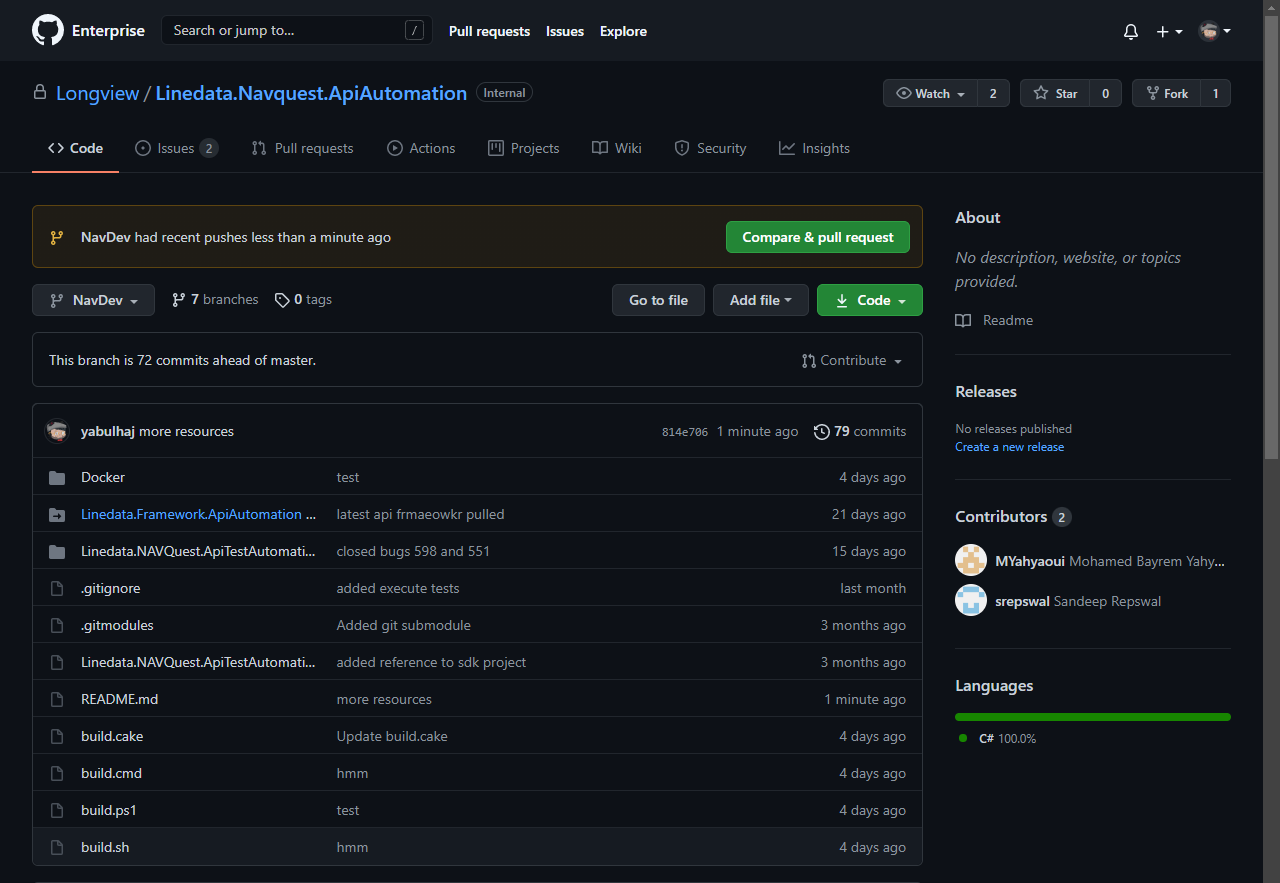
\includegraphics[width=.9\columnwidth]{Rapport ISTIC/p1.png}\\
\newline
\textbf{Part of the documentation:}\newline

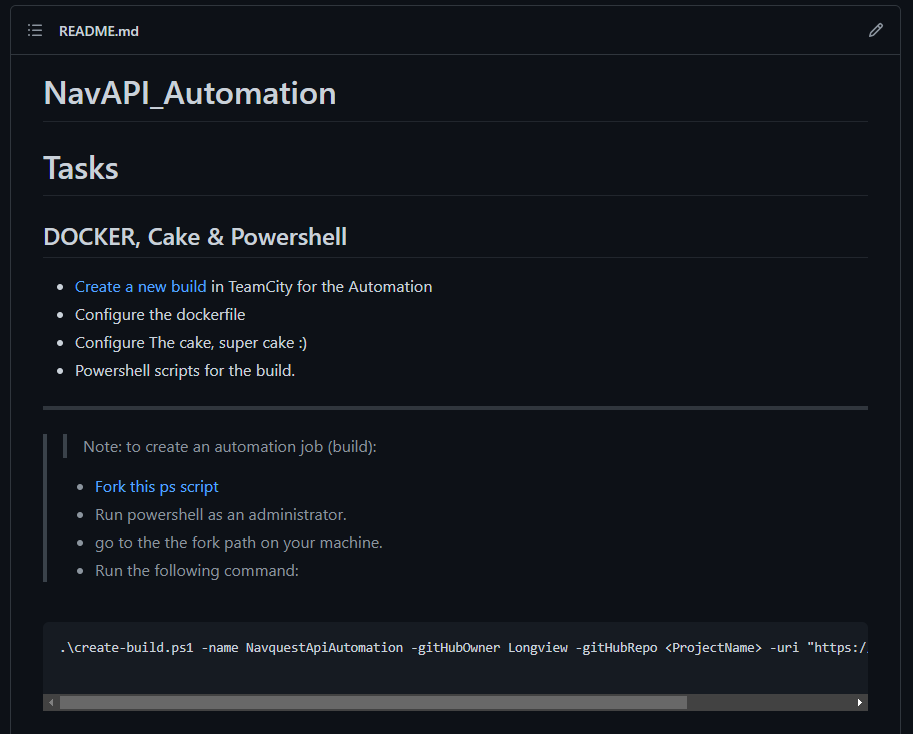
\includegraphics[width=.9\columnwidth]{Rapport ISTIC/p2.png}\\

\subsection{HARNESSIO}
Rather than real scripting, Harness uses a model to define your goals. Although you can use YAML within Harness, you do not need to write a script for the pipeline. The real advantage here is that you can simply select these steps, stages, and every component required for the configuration file using a user-friendly interface. I worked with colleagues to script the pipeline using the UI with HARNESS.\newline

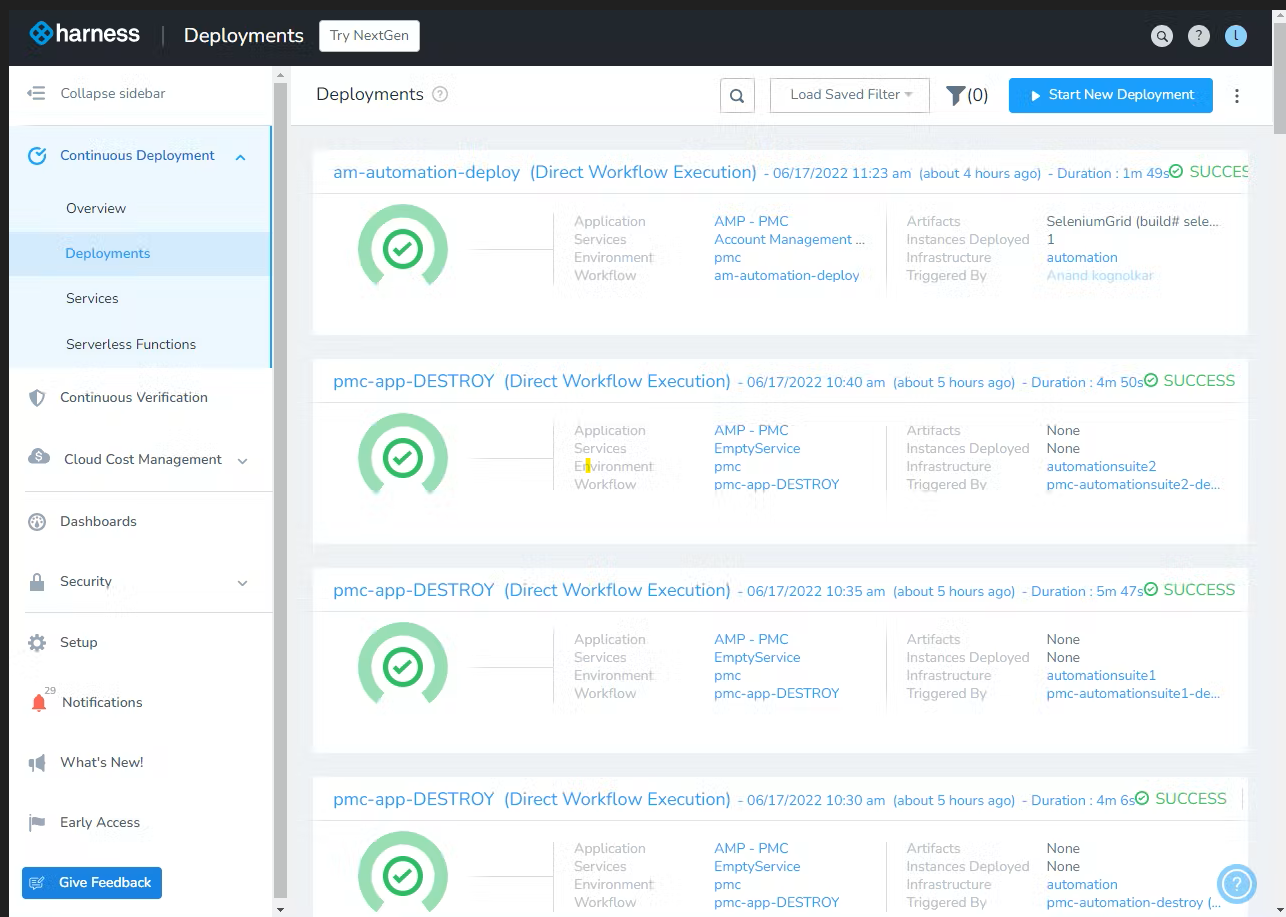
\includegraphics[width=1\columnwidth]{Rapport ISTIC/har.png}\\

\subsection{KUBERENETES}

Linedata is built entirely on the powerful container orchestration tool kubernetes. As earlier described, containers and docker are critical components. K8s simply make it easier to manage a large number of them. I spent a considerable amount of time managing the clusters, which included the pods that ran the containerized apps.\newline

Some of the tasks were as followed:
\begin{itemize}
  \item Install and Set Up kubectl on Windows.
  \item Certificate Management with kubeadm.
  \item Upgrading Windows nodes.
  \item Migrate Docker Engine nodes from dockershim to cri-dockerd.

\end{itemize}
\include{Chapitre4}
\chapter*{CONCLUSION AND FUTURE CAREER}
\addcontentsline{toc}{chapter}{General Conclusion}

\section{CONCLUSION}

Today's economic crisis affects everyone in the Tunisia, especially young adults who have just graduated from high school and are preparing for a life on their own. So the most important question for any young person is what they want to do with their lives. It is significant because if we make the wrong choices, we will waste our money, our time, and possibly our mental and physical health. However, we may not know whether the path we chose is the right one until later in life. Right now, I am confident in my decision to become a cloud obsessed.


However, in order to ensure the long-term success of Cloud Computing, the chapter addresses some significant challenges that the Cloud paradigm faces. User privacy, data security, data lock-in, availability, disaster recovery, performance, scalability, energy efficiency, and programmability are all issues that must be carefully addressed in future research.

\section{Further Career}
The demand for Cloud Computing professionals is expected to grow exponentially as more and more businesses implement this technology.
I have a strong belief in my vision, and I intend to continue on my path to become the best I can be by utilizing these user-friendly services and adding value to the world. The cloud will undoubtedly provide me with the ability to accomplish things on a large scale.


\begin{flushright}\LARGE
\bf{Thank you for reading.}
\end{flushright}





% Fin du document
\end{document}